\documentclass[final,3p,twocolumn]{elsarticle}

\usepackage{xcolor}
\definecolor{darkblue}{rgb}{0,0,0.5} 
\usepackage{transparent}
\usepackage{graphicx}
\usepackage{amsmath}
\usepackage{natbib}
\usepackage[colorlinks=true,
        urlcolor=darkblue,
        anchorcolor=darkblue,
        linkcolor=darkblue,
        citecolor=darkblue,
        pdfauthor={Johan B. C. Engelen},
        pdfkeywords={SVG; LaTeX; Inkscape},
        pdftitle={How to include an SVG image in LaTeX},
        pdfsubject={Describes how to include an SVG image easily in LaTeX using Inkscape}] {hyperref}
\usepackage{url}
\usepackage[protrusion=true,expansion=true]{microtype}

%\usepackage[T1]{fontenc}
%\usepackage[adobe-utopia]{mathdesign}
\usepackage{fourier}

\usepackage{calc}

\usepackage{verbatim}
\makeatletter
\g@addto@macro\@verbatim\small
\makeatother 

\newcommand{\executeiffilenewer}[3]{%
 \ifnum\pdfstrcmp{\pdffilemoddate{#1}}%
 {\pdffilemoddate{#2}}>0%
 {\immediate\write18{#3}}\fi%
}

\newcommand{\includesvg}[1]{%
 \executeiffilenewer{#1.svg}{#1.pdf}%
 {inkscape -z -D --file=#1.svg %
 --export-pdf=#1.pdf --export-latex}%
 \input{#1.pdf_tex}%
}
\begin{document}
\begin{frontmatter}

\title{How to include an SVG image in \LaTeX}

\author{Johan B. C. Engelen}
\address{\href{mailto:j.b.c.engelen@alumnus.utwente.nl}{j.b.c.engelen@alumnus.utwente.nl}}

\journal{\hspace{-10em}XXXXXXXXXXXXXXXX}

\begin{abstract}
How to make a \LaTeX\ document with vector images, where the text in the images has exactly the same font and size as in normal text?
This article describes how this is done using the `PDF/EPS/PS + LaTeX' output feature of Inkscape 0.48. Inkscape can export the graphics to PDF/EPS/PS, and the text to a \LaTeX\ file. When the \LaTeX\ file is input in the \LaTeX\ document, the PDF/EPS/PS image is included with overlaid text.
Because typesetting of the text is done by \LaTeX, \LaTeX\ commands can be used in images, such as writing equations, references and shorthand macros.\\
\emph{(requires Inkscape version 0.48 or higher; this document discusses features up to Inkscape 0.49)}
\end{abstract}
%
%\begin{keyword}
%LaTeX \sep SVG \sep Inkscape \sep PDFLaTeX
%\end{keyword}
\end{frontmatter}

%##########################################################################

\begin{figure}
\centering
  \executeiffilenewer{image.svg}{image-normal.pdf}{inkscape -z -D --file=image.svg --export-pdf=image-normal.pdf}
  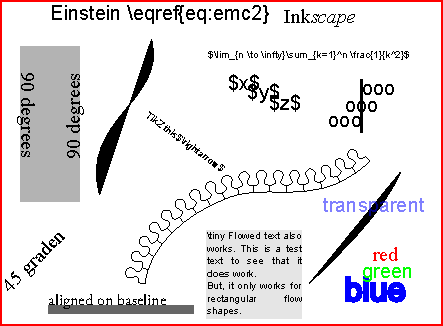
\includegraphics[width=\columnwidth]{image-normal.pdf}
  \caption{The test SVG image, as it is seen in Inkscape (exported to PDF \emph{without} \LaTeX\ option).}
  \label{fig:normal} 
\end{figure}

\begin{figure} 
\centering
  \def\svgwidth{\columnwidth}
  \includesvg{image}
  \caption{The test image, exported to PDF \emph{with} \LaTeX\ option.}
  \label{fig:pdflatex} 
\end{figure}

\section{Introduction}
An advantage of `drawing' images in \LaTeX\ code using e.g. TikZ, is the more uniform layout of the document as the image text will be typeset by \LaTeX: the image font will be equal to the rest of the document (size, ligatures, etc.). Moreover, TikZ enables easy use of mathematical expressions inside images. But, the programming nature of drawing with TikZ is not liked by many, and most will turn to a vector graphics drawing program, such as Inkscape. However, then, obtaining the document's font and mathematical expressions in images becomes a problem.
 
Inspired by the `epslatex' GNUPlot output terminal, a new feature was added to Inkscape, combining the advantages of \LaTeX\ text typesetting and drawing in Inkscape. This article describes how to use Inkscape to create images in which the text font is equal to the document's font, \LaTeX\ mathematical expressions can be written, and \LaTeX\ commands can be used. 
The automated inclusion of SVG graphics while using the new `PDF+LaTeX' Inkscape option is described.

\emph{(This article assumes the use of pdf\LaTeX\, but most will probably work just as well for EPS/PS documents.)}

\section{Creating the image with Inkscape}

The image can be drawn as usual in Inkscape, see figure~\ref{fig:normal}. All text in the image will be compiled by \LaTeX, and therefore may contain \LaTeX\ commands. For example, it is possible to refer to 
\begin{equation}
  E = mc^2.	\label{eq:emc2}
\end{equation}
Font type and size do not matter and will not be exported to \LaTeX.

\subsection{Text alignment}
I have tried to get the positioning of text in the end result as close as possible to the positioning in the SVG file. Text is aligned on the anchor point visible in Inkscape. This means that vertically, the baseline of the resulting text corresponds to the baseline of the text in Inkscape. Horizontally, it depends on the alignment (left, center, right).

\subsection{Text colour}
Text colouring works. If the text has a fill colour, this colour will be exported to \LaTeX\ as an RGB colour. Although stroking text will not work in \LaTeX, when the text as a stroke colour \emph{and no fill colour}, the stroke colour will be exported to \LaTeX\ as an RGB colour as if the text had that colour as fill. Text transparency is exported too.\footnote{Transparency is not exported when exporting to EPS or PS, because it is not supported by those formats.}

\subsection{Font shape (added in Inkscape 0.49)}
 Italic, oblique and bold text in Inkscape is exported to \LaTeX\ in a clause with {\small\verb|\textit{}|}, {\small\verb|\textsl{}|} or {\small\verb|\textbf{}|}, respectively.
Note that Arial has an oblique shape in Inkscape, instead of italic. This means that the \LaTeX\ file will contain {\small\verb|\textsl{}|}, and the result is a slanted font shape. If you want italics in your \LaTeX\ output, you should use a font that has italics in Inkscape (e.g. Times).

\subsection{Exporting to PDF}
When the image is saved to PDF, one has to set the `PDF+LaTeX' option in the dialog that pops up after specifying which file name to save to.
The bounding box of the image in Inkscape \emph{including text} will be used as the bounding box for the image if the exported area is the drawing ({\small\verb|--export-area-drawing|}). It is strongly recommended to use this `exported area is drawing' option, because text will not be clipped to the page size.

\subsubsection{Using Inkscape's command line}
\label{sct:cmdline}
Exporting to PDF and \LaTeX\ can also be performed through the command line interface:
{\small\ttfamily{inkscape -D -z --{}--file=image.svg --{}--export-pdf=image.pdf --{}--export-latex}}.
Note the added {\small\verb|--export-latex|} option.

\section{Including the image in \LaTeX}

The image should be included in the document by inputting the {\small\verb|.pdf_tex|} file created by Inkscape: 
\begin{verbatim}
\begin{figure} 
  \centering
  \def\svgwidth{\columnwidth}
  \input{image.pdf_tex}
\end{figure}
\end{verbatim}

The {\small\verb|.pdf_tex|} file created by Inkscape contains a {\small\verb|picture|} environment, that includes the PDF exported by Inkscape and places text on top of it. The result is figure~\ref{fig:pdflatex}, note that the font exactly matches the document's font, and the link to the equation works. 

\subsection{Scaling the image}
It is possible to set the width of the image by defining {\small\verb|\svgwidth|} before the {\small\verb|\input|} command:
\begin{verbatim}
\begin{figure} 
  \centering
  \def\svgwidth{\columnwidth}
  \input{image.pdf_tex}
\end{figure}
\end{verbatim}

One can also scale the image, by including the {\small\verb|calc|} package in the preamble and defining {\small\verb|\svgscale|} accordingly (\emph{added in Inkscape 0.48.2}):
\begin{verbatim}
\usepackage{calc}
...
\begin{figure} 
  \centering
  \def\svgscale{1.5}
  \input{image.pdf_tex}
\end{figure}
\end{verbatim}

Both {\small\verb|\svgwidth|} and {\small\verb|\svgscale|} are undefined (`forgotten') after including a figure ({\small\verb|\svgwidth|} and {\small\verb|\svgscale|} are set empty by {\small\verb|image.pdf_tex|}).

\subsection{When images are not in the document's directory}
When images are not located in the document's directory, but in a sub-directory, one has to add that directory to the graphics search path (unfortunately). For example, if one's images are in sub-directory {\small\verb|images|}, add the following to the preamble:
\begin{verbatim}
\graphicspath{{images/}}
\end{verbatim}

Alternatively, when the images are not in a sub-directory of the document, they can be accessed with the {\small\verb|import|} package, adding
\begin{verbatim}
\usepackage{import}
\end{verbatim}
to the preamble, and including the image with
\begin{verbatim}
\import{<path>/<to>/<file>}{<filename>.tex}
\end{verbatim}

\subsection{Automatic export}

(`write18' must be enabled, see the {\small\verb|epstopdf|} package documentation. Add {\small\verb|-shell-escape|} to the command line when calling {\small\verb|pdflatex|}.)

\subsubsection{Workflow}
Whenever the SVG file is updated, it is possible to have \LaTeX\ automatically call Inkscape to export the image to PDF and \LaTeX\ again. This simplifies the workflow to
\begin{itemize}
	\item Modify the SVG image in Inkscape;
	\item Save the SVG (Ctrl+S, no need to export to PDF);
	\item Recompile \LaTeX\ document. pdf\LaTeX\ will notice the SVG file has changed, and will automatically do the export for you.
\end{itemize}

\subsubsection{\LaTeX\ code}
Add the following code to the preamble of your document:
\begin{verbatim}
\newcommand{\executeiffilenewer}[3]{%
 \ifnum\pdfstrcmp{\pdffilemoddate{#1}}%
 {\pdffilemoddate{#2}}>0%
 {\immediate\write18{#3}}\fi%
}
\newcommand{\includesvg}[1]{%
 \executeiffilenewer{#1.svg}{#1.pdf}%
 {inkscape -z -D --file=#1.svg %
 --export-pdf=#1.pdf --export-latex}%
 \input{#1.pdf_tex}%
}
\end{verbatim}

When an image is included via {\small\verb|\includesvg|}, it is automatically exported to PDF+LaTeX again by Inkscape when the SVG file has changed (note that the image must be specified \emph{without} file extension):
\begin{verbatim}
\begin{figure} 
  \centering
  \def\svgwidth{\columnwidth}
  \includesvg{image}
\end{figure}
\end{verbatim}

The preamble code will only work if Inkscape is in the search path of your operating system (Windows: \url{http://www.computerhope.com/issues/ch000549.htm}).


\section{Example of using another font}
\fontfamily{phv}\selectfont
\renewcommand{\rmdefault}{phv}\rmfamily
When another font is chosen, the image font will of course also change to this font.
This is shown in figure~\ref{fig:otherfont}, where the same image file is included as in figure~\ref{fig:pdflatex}.

\begin{figure}[!h]
\centering
  \def\svgwidth{\columnwidth}
  \includesvg{image}
  \caption{The test image, exported to PDF \emph{with} \LaTeX\ option. Note that the image's font matches the newly chosen font. The included \LaTeX\ file is the same as in figure~\ref{fig:pdflatex}.}
  \label{fig:otherfont} 
\end{figure}

% switch back to Utopia
\fontfamily{put}\selectfont
\renewcommand{\rmdefault}{put}\rmfamily

\section{Known bugs and limitations}
It is advisable to use the latest Inkscape release, as additional features may have been added and bugs are continuously found and fixed.
Please report any bug you find on \url{https://bugs.launchpad.net/inkscape}.

There are still some known limitations/bugs. 
\begin{itemize}
  \item  Exporting to EPS+LaTeX, the bounding box is always set snugly around the drawing \emph{without} text. There is debate about whether this is a bug in Inkscape or not. This becomes a problem when text is desired `outside' the other parts of the drawing. A workaround is drawing a rectangle with zero stroke width as bounding box around the drawing. Alternatively, one can export to PS+LaTeX instead and renaming the resulting {\small\verb|.ps|} file to {\small\verb|.eps|}. See \url{https://bugs.launchpad.net/inkscape/+bug/595821}.
	\item  Flowed text is only exported for rectangular flow shapes.
  \item  The height of the figure cannot be specified.
  \item  It is not possible to use newlines in unflowed text.
\end{itemize}

\end{document}

